\documentclass[12pt, a4paper, oneside]{book}
\usepackage[french]{babel}
\usepackage[T1]{fontenc} 
\usepackage{lmodern} 
\usepackage[utf8x]{inputenc}
\usepackage{graphicx}
\usepackage{caption}
\usepackage{hyperref}
\usepackage{natbib}
\usepackage[ruled,french,lined,algonl,boxed]{algorithm2e}
\usepackage{fancyhdr}
\usepackage{hyperref}
\usepackage{array,multirow,makecell}
\usepackage{fancybox}
\usepackage{boxedminipage}
\usepackage{graphicx}
\usepackage{epstopdf}

\newtheorem{Def}{\textbf{\textsc{Définition}}}
\newtheorem{Exp}{\textbf{\textsc{Example}}}
\newtheorem{Rq}{\textbf{{Remark}}}
\newtheorem{Prop}{\textbf{Proposition}}
\newtheorem{Lemme}{\textbf{Lemme}}


%\setcounter{secnumdepth}{6}
\newcolumntype{R}[1]{>{\raggedleft\arraybackslash }b{#1}}
\newcolumntype{L}[1]{>{\raggedright\arraybackslash }b{#1}}
\newcolumntype{C}[1]{>{\centering\arraybackslash }b{#1}}
%\renewcommand{\thesubsubsection}{\int{subsubsection}}
%\renewcommand{\thechapter}{\Roman{chapter}}
%\renewcommand{\thesection}{\Latin{section}}
\pagestyle{plain}
\bibliographystyle{plain}

\begin{document}
\frontmatter
\listoffigures
\tableofcontents
%\pagenumbering{gobble}

\mainmatter

\chapter{Introduction générale}

L'intelligence artificielle (IA) a vu son importance s'accroître considérablement
par sa capacité à s'attaquer à de nouvelles classes de problèmes, différents de ceux
traités par l'informatique classique. Ces problèmes relèvent d'activités humaines
variées (perception, prise de décision, planification, diagnostic, interprétation de
données, compréhension du langage, conception, etc.) et nécessitent l'exploitation d'une grande quantité de connaissances.\citep{IA}

\paragraph{}

Puis, avec l'avènement du web et les avancées technologiques, un intérêt
particulier de l'IA, pour une structuration du sens et une gestion automatique et
intelligente du contenu du web est apparu. Ceci s'inscrit dans le cadre d'une
application concrète de grande envergure, le Web Sémantique. \citep{avenement}

\paragraph{}

L'idée initiale derrière le web fut de pouvoir gérer une quantité volumineuse de données et documents, liés les uns aux autres. La difficulté de cette approche résidait dans le fait qu'il fallait dans certaines situations, parcourir tous les documents pour finalement atteindre l'information souhaitée.



\paragraph{}

Après cela, arrivèrent les hyperliens (hyperlinks en anglais) qui consistent en un seul clic, à accéder 
au document souhaité, et c'est à partir de là que le mot "Web" a réellement pris tout son sens.



\paragraph{}

Cependant, les données présentes sur le Web ne peuvent êtres interprétées que par l'homme. En effet, les algorithmes ne peuvent pas comprendre les données afin de les étudier et de les manipuler.
\paragraph{}
A partir de ce constat, le W3C (World Wide Web Consortium) se tourna vers un web qui a pour objectif de fournir des informations pertinentes aux utilisateurs et donner un sens aux données présentes, le nommément Web Sémantique (Semantic web en anglais).
\paragraph{}
Dans le cadre de mon alternance au sein d'Axa Assurance, il m'est souvent arrivé de devoir naviguer dans le réseau d'Axa pour me documenter et rechercher des informations bien précises.
\paragraph{}

Le réseau d'Axa a pour particularité d'être très riche en terme de documents présents.
Cependant, ces derniers sont difficilement trouvables.


C'est ainsi que l'idée de concevoir et réaliser une application de recherche et de documentation basée sur le Web Sémantique m'est venue.


\paragraph{}
Dans le but de permettre une recherche ne se basant pas uniquement sur les mots clés, une recherche qui donnerait du sens aux données, j'ai choisi d'articuler mes travaux autour du Web Sémantique et des outils et moyens qu'il présente. 


J'ai choisi d'illustrer l'approche proposée à travers une application liée à la recherche dans le domaine des assurances tel que : la souscription, les clauses, les contrats et les tarifs nationaux.  





\paragraph{}
J'organise ainsi mon mémoire : 


\chapter{Contexte et problématique}
\section{Description du contexte}

\paragraph{}

Avant de détailler la problématique de ce travail, il est tout d'abord important d'évoquer le contexte, ainsi que les facteurs ayant fait que celle ci voit le jour et devienne un sujet de recherche.

\paragraph{}

Me concernant, tout a commencé lors de mon stage de master 1 auprès d'AXA France, au sein de la Branche Transports IARD.


\paragraph{}

Pour rappel, Axa est un groupe international français spécialisé dans l'assurance depuis sa création, en 1982, et dans la gestion d'actifs depuis 1994. La marque AXA a été la première marque mondiale d'assurance pour la 9e année consécutive.


\paragraph{}

Il est souvent difficile de décrire l'organigramme d'une structure aussi
grande et complexe que celle d'AXA. Néanmoins, il est important de préciser que la branche Transports est un service faisant partie de l'organisation d'Entreprise d'AXA.

\paragraph{}

La branche Transports d'AXA France accompagne ses clients professionnels à faire face aux aléas de la vie en proposant 3 types de contrats selon les besoins du client.


\paragraph{}

A mon arrivée le 04 Juin 2018 au sein de la Branche Transports, en tant que stagiaire chargé de projet informatique, j'avais pour principales missions d'analyser les besoins informatiques de la Branche et de développer des outils d'aide à la gestion et à la souscription.


\paragraph{}

Assurer de telles missions nécessitait des connaissances approfondies dans le domaine des assurances, domaine que je n'avais pas exploré auparavant.

\paragraph{}
Il était donc nécessaire de bien me documenter à ce sujet et ce, dans le but de garantir une meilleure compréhension des processus de souscription aux assurances et de les optimiser.

\paragraph{}

Mon maître d'apprentissage me conseillait de naviguer sur le réseau d'Axa France afin de trouver des réponses à mes différentes questions liées aux assurances. 
 
\paragraph{}

Le réseau d'Axa France a pour particularité d'être : 

\begin{itemize}
\item Très vaste en terme de documents disponibles.
\item Peu structuré.
\item Accessible par tous les collaborateurs (Lecture et écriture publique).
\end{itemize}

 
\paragraph{}
La recherche était de ce fait très laborieuse et difficile
\paragraph{}
C'est à partir d'un tel constat que l'idée de munir le réseau d'Axa d'un moteur de recherche plus précis a émergé.


\paragraph{}
Ce moteur de recherche aurait la particularité d'assimiler les termes donnés en entrée et de leur attribuer une sémantique (sens) et cela dans l'objectif de rendre les résultats meilleurs et plus pertinents.


\paragraph{}
C'est dans ce contexte alors que la problématique de mon mémoire a été formulée : 

\paragraph{}
\emph{\textbf{Comment créer un moteur de recherche sémantique dans le réseau d'Axa France ?} 
}

\paragraph{}
Cependant, plusieurs questions peuvent découler d'une telle problématique, je cite : 

\begin{enumerate}


\item Quels sont les principes de base du Web Sémantique ?
\item Qu'est ce qu'une ontologie ?  Et pourquoi son rôle est-il primordial dans la recherche sémantique ? 
\item Comment générer une ontologie automatiquement à partir des documents non structurés se trouvant dans le réseau d'Axa ? 


\end{enumerate}



\paragraph{}
Tout au long de ce document, nous essayerons de répondre de manière systémique et analytique à la problématique énoncée, ainsi qu'aux différentes questions qui en dérivent. 

\pagebreak

\section{Pourquoi avoir choisi cette problématique ?}

\paragraph{}
La connaissance de l'entreprise est un atout essentiel dans le monde économique et concurrentiel.
La capacité d'apprendre, de stocker et de diffuser des connaissances implicites et explicites peut déterminer le succès, ainsi que l'échec d'une entreprise souhaitant émerger. Bien que la gestion des connaissances en entreprise soit un domaine de recherche bien défini, les implémentations actuelles manquent d'orientation et  de méthodologie particulièrement dans les grands groupes.
\paragraph{}
Dans le contexte actuel, les grandes entreprises modernes ont besoin d'utiliser des pratiques qui leurs sont propres.
Comme de plus en plus d'employés deviennent des "travailleurs du savoir",
la connaissance est générée de manière très rapide et massive à la fois.
\paragraph{}
Dans ce contexte intervient le knowledge management , en veillant à ce que le savoir développé au sein de l'entreprise soit pérennisé et préservé.
\paragraph{}
L'une des méthodes employées consiste à fournir un maximum de documents afin que le turn-over des employés au sein d'un service n'impacte pas brutalement l'activité de ce dernier.
\paragraph{}
Par ailleurs, cela rejoint les problématiques des entreprises modernes qui sont constamment à la recherche de solutions pour palier au problèmes liés à la documentation des nouveaux collaborateurs et comment faciliter l'apprentissage du métier à leurs débuts.
\paragraph{}
Le Web sémantique est un domaine répondant à la problématique liée à la classification des documents selon leur domaine (Thématique) et à la recherche sémantique de ces derniers.
\paragraph{}
Il s'agit d'un domaine qui m'a beaucoup intéressé, particulièrement après avoir lu des articles en Master 1, lors de mon projet d'ingénierie et de représentation des connaissances (Knowledge representation) suivi à Dauphine.
\paragraph{}
De plus, le thème de ce mémoire a suscité l'intérêt de plusieurs personnes de mon entourage. Je cite mon maître d'apprentissage chez Axa France, qui s'intéresse beaucoup aux problématiques liées à la recherche de documents.
\paragraph{}
C'est à partir de ces éléments que j'ai pris la décision d'orienter mon mémoire vers un sujet certes très orienté recherche, mais qui répondrait à une vraie problématique rencontrée dans n'importe quelle entreprise possédant une large bibliothèque de documents.
\paragraph{}
J'estime que le Web Sémantique est, et sera la prochaine tendance de toutes les applications informatiques nécessitant l'interprétation de la donnée en information pour rendre les résultats plus précis et les algorithmes plus intelligents.


\chapter{État de l'art}
\section{Introduction}

\paragraph{}
Le Web sémantique désigne, en premier lieu, une activité du W3C.
Le mot “sémantique” ne renvoie pas à la définition communément admise en linguistique, mais fait référence à la définition donnée par le domaine de la logique de description dont le but est de faire émerger du sens à travers les données. Il s'agit en effet de donner un sens aux données employées \citep{w3c}.
\paragraph{}
Plusieurs définitions ont été proposées dans la littérature, nous choisissons celle présentée par Tim Berners-lee dans le magazine “Scientific American”, "The Semantic Web is an extension of the current web in which information is given well-defined meaning, better enabling computers and people to work in cooperation.". \citep{defOnto}
\paragraph{}
Ce qui signifie que le web sémantique est une extension du web actuel dans lequel l'information est pourvue d'un sens bien défini permettant une coopération entre l'homme et la machine. 
\paragraph{}
Au cours de ce chapitre, je donne un aperçu sur les aspects fondamentaux de la représentation des connaissances et sur les ontologies, ainsi que leur impact sur l'intelligence artificielle.
\paragraph{}
Ce chapitre est ensuite complété par un état de l'art sur les solutions existantes liées à la problématique énoncée.

\section{Notions de base du Web Sémantique}

\subsection{Représentation des connaissances}
\paragraph{}
Représenter des connaissances propres à un domaine particulier consiste à décrire
et coder les entités du domaine sous une forme exploitable par un système
informatique, pour mener à bien des raisonnements et résoudre des problèmes dans le
domaine étudié \citep{kayser}.
\paragraph{}
La représentation des connaissances est l'application
de la logique et l'ontologie dans un but de construire des modèles calculables pour
certains domaines (Sowa, 2000).
\paragraph{}
Autrement dit, la représentation des connaissances consiste à formaliser les données de façon logique et mathématique afin que la machine puisse les interpréter en informations, permettant de ce fait d'assurer une inférence des données, conduisant à un comportement cognitif.


\subsection{Architecture du Web Sémantique}
\paragraph{}
Tim Berners Lee a décrit le Web Sémantique suivant l'architecture tel indiqué dans la figure \ref{couches} :  

\begin{figure}[h!]
\begin{center}
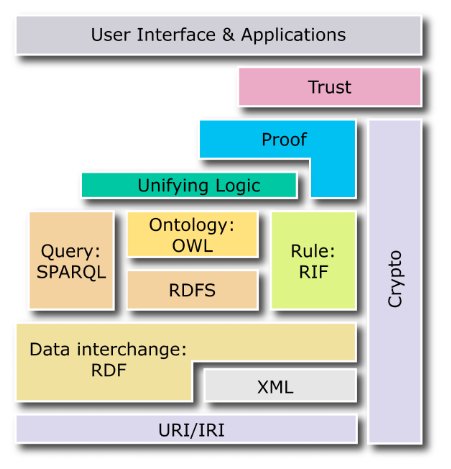
\includegraphics[scale=0.6]{/home/boukala/Bureau/Memoire/figures/couches.png}
\caption{Architecture du Web Sémantique}
\label{couches}
\end{center}
\end{figure}


\begin{enumerate}

\item \textbf{Niveau d'adressage : } On y retrouve l'Unicode ainsi que l'URI.

\item \textbf{Niveau syntaxique : } On y retrouve le code XML (eXtensible Markup Language) qui fournit une syntaxe élémentaire pour la structure des documents.

\item \textbf{Niveau sémantique : } Qui représente l'ensemble des fondamentaux du web sémantique.

\end{enumerate}

\paragraph{}
Dans ce document, je m'intéresse particulièrement aux éléments constituant le niveau sémantique. Il s'agit des ontologies et des bases RDF.


\subsection{Concepts de base du Web Sémantique}
\paragraph{}
Dans le but de donner du sens aux données utilisées dans le Web, différents outils sont mis à disposition afin d'identifier les données facilement sans se soucier du stockage de ces dernières et des documents où elles sont contenues.
\paragraph{}
Ces outils sont présentés dans ce qui suit :
\begin{itemize}
\item Un moyen d'identifier les données à travers le web de manière unique (les URIs).
\item Un moyen de configurer des relations avec d'autres données(Les bases RDF).
\item Un moyen de comprendre ce que sont ces relations (le vocabulaire).
\end{itemize}

\subsection{URI (Unified Resource identifier)}
\paragraph{}
Permet d'adresser les données de manière unique. 
Ainsi, deux données différentes ne peuvent pas avoir le même URI.
Un exemple d'URIs les plus fréquents sont les URLs.
\paragraph{}
Ce concept est fondamental dans le web sémantique.
Il met en évidence certaines lacunes lors de l'utilisation des bases de données relationnelles.
Par exemple, nous utilisons des clés primaires pour identifier chaque information. Cependant, nous pouvons avoir la même clé primaire dans deux bases de données différentes et qui n'identifient pas la même donnée. 
En revanche, l'utilisation des URIs nous garantit qu'une donnée référencée par un URI est toujours la même, ainsi la machine n'aura pas à traiter des données ambiguës.

\subsection{Modèle RDF (Resource Description Framework)}
\paragraph{}
(RDF) est un modèle de graphe destiné à décrire de façon formelle les ressources Web et leurs métadonnées, de façon à permettre le traitement automatique de telles descriptions. 
\paragraph{}
Développé par le W3C, RDF est le langage de base du Web sémantique. L'une des syntaxes (ou sérialisations) de ce langage est RDF/XML. D'autres syntaxes de RDF sont apparues ensuite, cherchant à rendre la lecture plus compréhensible ; c'est le cas par exemple de Notation3 (ou N3).
\paragraph{}
En annotant des documents non structurés et en servant d'interface pour des applications et des documents structurés (par exemple bases de données) RDF permet une certaine interopérabilité entre des applications échangeant de l'information non formalisée et non structurée sur le Web.
\paragraph{}
Le modèle RDF est issu de la réflexion sur la théorie des graphes et la logique des prédicats. 
En effet, en RDF, les relations qui unissent deux entités sont orientées d'où la dénomination de graphe orienté et sont typées d'où la relation avec la logique des prédicats du premier ordre et est considéré comme étant le langage de base du web sémantique pour les données. 
\paragraph{}
Tout document RDF est composé d'un ensemble de triplets. Un triplet est décrit de la manière suivante :
\paragraph{}
\textbf{“Sujet” Prédicat “Objet”}
\paragraph{}

\begin{itemize}

\item \textbf{Le sujet : }ressource décrite par RDF qui peut être une page web ou un objet quelconque et est représenté par une URI (Uniforme Ressource Identifier) unique.
\item \textbf{Le prédicat (propriété) : }représente une relation entre des ressources.
\item \textbf{L'objet : }représente la valeur de la propriété. Si l'objet du triplet RDF est un URI alors
l'objet est considéré comme une ressource qui peut être utilisée dans un autre triplet en tant
que sujet, sinon (cas ou l'objet est sous forme littéral ) il ne peut plus être utilisé.

\end{itemize}

\paragraph{}
Il existe plusieurs façons de représenter une relation RDF. On parle alors de langage formel de représentation. Nous citons : RDF/XML, Turtle NTriple … .
\paragraph{}
Ces langages permettent de représenter les données de manière assez claire et intuitive.
Nous pouvons aussi modéliser une relation RDF à l'aide d'un graphe orienté comme indiqué précédemment.

\paragraph{}
Ces graphes sont représentés de la manière suivante : 


\paragraph{}
Un graphe orienté et étiqueté où les sujets sont représentés par des nœuds. Les nœuds sont sous forme de cercle pour les URI.
Les arcs quant à eux, sont étiquetés par des prédicats.

\paragraph{}

\begin{figure}[h!]
\begin{center}
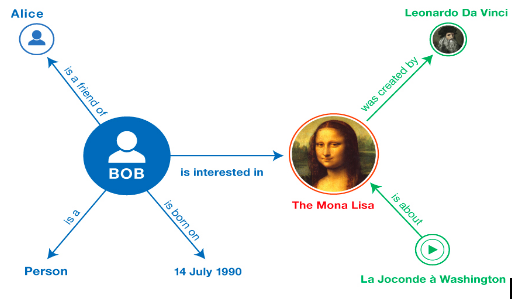
\includegraphics[scale=0.6]{/home/boukala/Bureau/Memoire/figures/exempleRDF.png}
\caption{Exemple de graphe RDF}
\end{center}
\end{figure}


Notons que dans cet exemple, “Bob” représente le sujet, “Is interested in” la relation et “The Mona Lisa” le prédicat qui lui même est aussi le sujet  pour d'autres relations.

\subsection{Ontologies}

\subsubsection{de l'Ontologie à l'ontologie}
\paragraph{}
Le terme « ontologie », construit à partir des racines grecques ontos (ce que existe, l'existant) et logos (le discours, l'étude), est un mot que l'informatique a emprunté à la philosophie au début des années 1990. 
\paragraph{}
En philosophie, l'Ontologie ( avec un O majuscule) est une branche fondamentale de la Métaphysique, qui s'intéresse à la notion d'existence, aux catégories fondamentales de l'existant et étudie les propriétés les plus générales de l'être.

Référence : https://interstices.info/ontologies-informatiques/

\subsubsection{L'ontologie d'un point de vue informatique}

\paragraph{}
Une ontologie en informatique est un ensemble structuré de concepts permettant de donner un sens aux informations.(référence https://www.institut-numerique.org/21-les-ontologies-51f7a7f9e921c)
\paragraph{}
 Son objectif premier est de modéliser un ensemble de connaissances dans un domaine donné, permettant ainsi de représenter un corpus de connaissances sous forme utilisable par un ordinateur.
\paragraph{}
Les ontologies sont employées dans l'intelligence artificielle, le Web sémantique, le génie logiciel, l'informatique biomédicale et l'architecture de l'information comme une forme de représentation de la connaissance. 
\paragraph{}
Les ontologies décrivent généralement les :
\begin{itemize}
\item \textbf{Individus} : objets de base,
\item \textbf{Classes} : ensembles, collections, ou types d'objets,
\item \textbf{Attributs} : propriétés, fonctionnalités, caractéristiques ou paramètres que les objets peuvent posséder et partager,
\item \textbf{Relations} : liens que les objets peuvent avoir entre eux,
\item \textbf{Évènements} : changements subis par des attributs ou des relations.
\end{itemize}

\paragraph{}
Le graphe suivant représente un exemple d’ontologie :

\begin{figure}[h!]
\begin{center}
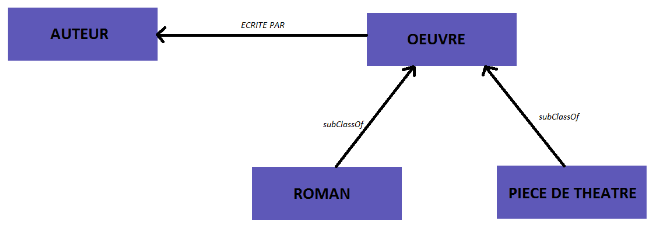
\includegraphics[scale=0.6]{/home/boukala/Bureau/Memoire/figures/exempleOntologie.png}
\caption{Exemple d'ontologie sous forme de graphe}
\end{center}
\end{figure}






\subsubsection{Représentation des ontologies}
\paragraph{}
Le problème posé par la représentation des connaissances est de pouvoir trouver un langage formel permettant de modéliser toutes les informations souhaitées et confondues.
\paragraph{}
Un langage formel se construit à partir d'un alphabet comprenant des symboles de variables (identificateurs), des symboles de fonction, des symboles de prédicat et des symboles d'opérateurs logiques (connecteurs), des quantificateurs, etc.
\paragraph{}
Ces symboles sont des primitives à partir desquelles toutes les formules bien formées du langage sont construites selon des règles de construction syntaxique reconnues par le langage lui-même (Analyse syntaxique de la compilation d'un langage formel). Mais il ne suffit pas de préciser comment construire les formules du langage, il faut en outre préciser quelle signification ou sémantique elles peuvent recevoir, pour leur associer des connaissances du domaine, d'où l'aspect sémantique que l'on souhaite introduire dans ce nouveau domaine.
\paragraph{}
C'est de cette manière que les ontologies sont représentées à l'aide d'un langage de représentation des connaissances, rendant ces dernières compréhensible par la machine.
\paragraph{}
Parmi les langages utilisés dans la représentation des ontologies, je cite : RDF(S), OWL et Logique de Description.
\paragraph{}
Dans ce qui suit, je présente le langage OWL qui offre une certaine puissance d'expression, permettant de décrire les ontologies de manière explicite et bien détaillée.

\subsubsection{Le Langage OWL}
\paragraph{}
OWL a été élaboré comme nouveau langage d'ontologies standard pour le web. Il repose sur RDFS et tente de trouver un équilibre entre puissance d'expression et support logique efficace. La logique (le raisonnement) est un facteur important parce qu'elle permet de :
\begin{itemize}
\item Vérifier la cohérence d'une ontologie et des connaissances.
\item Vérifier la présence de relations non voulues entre classes.
\item Classer automatiquement les instances.
\end{itemize}


\subsubsection{Composants d'une ontologie}
\paragraph{}
En informatique comme en philosophie, l'ontologie comprend plusieurs composants. Dans ce qui suit, je m'intéresse à ces composants :
\begin{itemize}
\item \textbf{Concept (également appelé classe) : }représentant un objet du monde réel, une idée, ou même une URI. Un concept n'a qu'un sens et une seule définition, ce qui permet d'éviter toute ambiguïté. Un concept est défini par :
\item \textbf{Terme : }exprimant le nom du concept.
\item \textbf{Attribut : }permet de spécifier et de donner des caractéristiques aux concepts par exemple : le concept 'étudiant' a un 'matricule', 'nom','prénom', etc.
\item \textbf{Instances ou extensions : }qui sont aussi appelées individus représentent les objets manipulés à travers les concepts ex : 'Dupont' est une instance de 'étudiant'.
\item \textbf{Relations : } les liens que les concepts ou même leurs instances peuvent avoir entre eux.
\end{itemize}

\subsubsection{Exemple d'ontologie}
\paragraph{}
Dans l'exemple illustré ci-dessus, il existe deux relations : subClassof et ECRITE PAR et 4 Concepts : ROMAN, PIECE DE THEATRE, OEUVRE et AUTEUR.

\paragraph{}
Au cours de cette première partie, nous avons introduit les notions de base du web sémantique nécessaires à la bonne compréhension du sujet abordé.
\paragraph{}
Dans ce qui suit, nous présentons de manière détaillée des solutions et architectures existantes dans la littérature, répondant à la problématique liée à la génération automatique des ontologies.
Ces solutions serviront par la suite lors de l'élaboration du moteur de recherche sémantique.

\newpage
\section{Solutions existantes}

\subsection{Ontology learning from Web-based corpus}

\paragraph{}
Dans cette partie, nous présentons une méthode basée sur l'apprentissage des ontologies de domaine\citep{inproceedings}. Il s'agit d'un composant primordial pour un moteur de recherche sémantique dans une entreprise, quelque soit sa structure et sa taille.
\subsubsection{Moteur de recherche sémantique basé sur les ontologies de domaine}
\paragraph{}
De manière générale, les moteurs de recherche ont pour objectif principal d'augmenter le résultat de deux ratios : \emph{Le taux de précision et le taux de rappel.} \citep{defOnto}

\paragraph{}
Ces deux paramètres sont définis de la manière suivante : 

\paragraph{}

\emph{Taux de précision = (Nombre de documents pertinentes retrouvés) / (Nombre de documents retrouvés)
}
\paragraph{}

\emph{Taux de rappel = (Nombre de documents pertinentes retrouvés) / (Nombre de documents pertinents)
}
\paragraph{}
Les moteurs de recherche sémantiques permettent d'augmenter considérablement les deux indicateurs ci-dessus en exploitant le contexte sémantique de la requête formulée avec la connaissance du domaine pertinent.
Cette connaissance de domaine est formalisée sous forme d'ontologie.

\paragraph{}
L'avantage d'utiliser un moteur de recherche sémantique basé sur les ontologies de domaine réside dans le fait que la requête formulée initialement, peut-être automatiquement réécrite en prenant en compte les éléments suivants \citep{avantage} : 

\begin{itemize}
\item Inclure les concepts qui sont en relation avec les termes (concepts) de la requête initiale
\item Découper les concepts dans la requête
\item Remplacer les concepts initiaux par les concepts qui sont en relation
\end{itemize}

\paragraph{}
Le graphe représentatif des ontologies peut-être utilisé pour déterminer la corrélation entre deux concepts différents. Par exemple, l'application d'algorithmes basés sur le plus court chemin pour déterminer si deux concepts c1 et c2, présents dans un même graphe G, sont en relation forte si et seulement si, la distance entre ces sommets est minimale.



\subsubsection{Apprentissage des ontologies (Ontology learning) }
\paragraph{}
Le problème majeur avec les ontologies de domaine est que ces dernières ne sont généralement pas disponibles dans la littérature car elles sont difficiles à développer manuellement. En effet, construire une ontologie manuellement nécessite des experts du domaine étudié, en plus des compétences informatiques. 
\paragraph{}
La méthode proposée dans cette solution consiste à générer des ontologies de domaine automatiquement. Ces dernières seront par la suite utilisées par le moteur de recherche sémantique pour garantir de meilleurs résultats.
\paragraph{}
La construction des ontologies se fera à partir de documents non structurés et ce, dans le but de généraliser le processus pour n'importe quel type de document.
\paragraph{}
Il est important de noter que l'apprentissage des ontologies pourra servir à la classification des documents en fonction des thématiques traitées dans les entreprises, ainsi qu'à la recherche sémantique.
\paragraph{}
Plusieurs algorithmes sont proposés pour implémenter l'ontology Learning. 
Dans cette solution, il s'agit de combiner des méthodes basées sur la machine Learning ainsi que, des algorithmes NLP. C'est d'ailleurs ce que nous retrouvons dans l'outil Text2Onto développé en Java, qui est utilisé dans l'architecture que je présente dans ce qui suit.

\subsubsection{Architecture du moteur de recherche proposé}
\paragraph{}
Le moteur de recherche sémantique présenté dans cette partie peut-être utilisé par n'importe quel employé à la recherche de documents bien spécifiques relatifs à l'entreprise.
\paragraph{}
L'architecture représentée ci-dessous décrit 3 principaux cas d'utilisations :
\begin{itemize}
\item La recherche d'un document
\item Construction et enrichissement de l'ontologie
\item Indexation du référentiel du document
\end{itemize}


\begin{figure}[h!]
\begin{center}
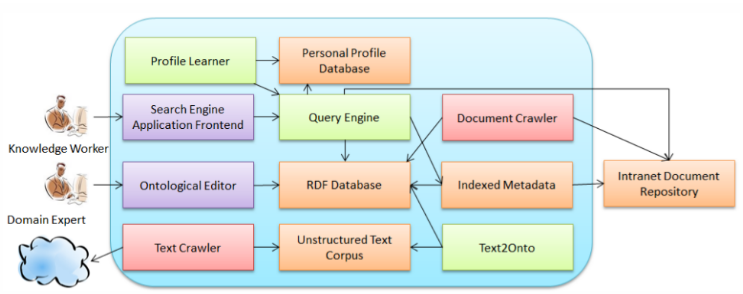
\includegraphics[scale=0.5]{/home/boukala/Bureau/Memoire/figures/architecture1.png}
\caption{Architecture du moteur de recherche sémantique proposé}
\end{center}
\end{figure}






\paragraph{}
Concernant la construction et l'enrichissement de l'ontologie, un composant appelé text Crawler component est utilisé.
\paragraph{}
Ce composant a pour objectif de chercher des documents à partir de sources publiques, sur la base d'un terme initial, par exemple : “Assurance”. Ce qui permet d'effectuer un traitement préliminaire.
Les documents retrouvés seront ensuite stockés dans un répertoire de documents non structurés.
\paragraph{}
C'est ensuite au tour du composant Text2Onto de parcourir le corpus de documents stockés et de générer automatiquement une Ontologie de domaine.
\paragraph{}
Il est cependant nécessaire qu'un expert du domaine puisse valider l'ontologie, que cette dernière est conforme au modèle attendu. Dans le cas échéant, l'expert aura la possibilité de la modifier à l'aide d'un composant appelé Ontological editor Component.
                                           
\subsubsection{Le composant de génération d'ontologies}
\paragraph{}
Comme indiqué précédemment, la génération automatique des ontologies est basée sur un outil open source Text2Onto.
\paragraph{}
L'utilisation de cet outil consiste dans un premier temps à renseigner manuellement des termes en relation avec le domaine traité. 
Cette étape permet de composer un corpus (Ensemble de documents pertinents et en relation avec la thématique choisie)
\paragraph{}
Dans le but d'évaluer la précision et la qualité du résultat obtenu par l'outil, la méthode suivante est appliquée :
\begin{enumerate}
\item L'Ontologie de domaine (Insurance par exemple) est générée automatiquement à l'aide de Text2Onto.
Chercher sur Swoogle l'ontologie Insurance \citep{swoogle}. La développer manuellement dans le cas où cette dernière n'est pas existante.
\item Évaluer la similarité entre les deux ontologies (1 et 2), à savoir celle générée automatiquement et celle développée manuellement. L'évaluation se fait en calculant l'indicateur Commun Concept que nous notons dans ce qui suit CC

\item L'indicateur CC est calculé de la manière suivante: $$CC (\%) = (No. common concepts) / (Total\;no. concepts in both ontologies)$$

\end{enumerate}




\paragraph{}
Ce calcul permet d'indiquer le nombre de concepts communs aux deux ontologies.
Le calcul du nombre de concepts en commun se fait suivant l'algorithme suivant : 

\begin{enumerate}

\item Pour chaque concept de l'ontologie 1, générer une liste L des concepts synonymes.
\item Pour chaque élément de L, parcourir l'ensemble des concepts de l'ontologie 2.
\item Tester la présence d'intersection entre les deux listes.

\end{enumerate}

\paragraph{}

L'utilisation de cet algorithme permet d'évaluer l'ontologie générée automatiquement en définissant un seuil d'acceptabilité de l'ontologie.

\subsubsection{Discussion}
\paragraph{}
Après avoir exposé cette première solution, il est important de faire le point quant aux avantages et aux inconvénients présents. 
\paragraph{}
L'architecture présentée offre des résultats intéressants dans la mesure où cette dernière utilise des API préalablement existantes, auxquelles des portions de code ont été intégrées dans le but d'affiner la recherche et la rendre plus pertinente.
\paragraph{}
Néanmoins, l'Ontologie de domaine générée automatiquement n'est pas aussi riche que ce que pourrait proposer un expert du domaine étudié.
\paragraph{}
Par conséquent, il est nécessaire de greffer des algorithmes de Datamining pour garantir des résultats convergeant vers une générations plus complètes. 
\paragraph{}
Dans ce qui suit, nous exposons une solution pour générer les ontologies, basée sur des outils de Datamining

\newpage
\subsection{Semantic search based on automatic building of an Ontology from a Corpus of Text Documents Using Data Mining Tools} 

\paragraph{}
Dans cette partie, nous présentons une procédure permettant de créer des ontologies automatiquement en utilisant des méthodes basées sur la fouille de données.\cite{article}
\paragraph{}
Il s'agira ensuite d'intégrer cette procédure dans un moteur de recherche sémantique.
\paragraph{} 
Il est toutefois important de noter que cette solution diffère de la solution présentée précédemment (Cf ) dans certains points de vue, à savoir : \\
\begin{itemize}
\item Utilisation de méthodes basées sur le datamining.
\item Le processus de création d'une nouvelle ontologie automatiquement ne nécessite pas l'intervention d'un expert.
\item Apprentissage supervisé pouvant garantir de meilleurs résultats.
\end{itemize}

\paragraph{} 
Un document non structuré peut décrire plusieurs concepts et relations à la fois.
Chaque concept peut-être désigné par N mots différents.
Il est ensuite nécessaire de trouver les relations liant les différents concepts pertinents retrouvés.\citep{process1}
\paragraph{} 
La difficulté d'un tel modèle réside dans le fait que nous ne pouvons pas avoir recours à une aide extérieure tel qu'un dictionnaire ou un expert du domaine. 
\paragraph{} 
Dans ce qui suit, nous exposons la méthodologie, ainsi que les algorithmes 
appliqués pour répondre à la problématique énoncée. 

\subsubsection{Étape préliminaire}

\paragraph{} 
Nous considérons un ensemble de documents sous format  PDF en entrée. Ces documents sont tous liés à une même thématique. Dans notre cas, il s'agit du domaine des assurances.\\
Ces documents passent par une étape d'extraction, de filtrage et de nettoyage.
\paragraph{} 
Pour ce faire, PDFBox est utilisé afin d'extraire le contenu du PDF en variable de type String (chaîne de caractères) \cite{apache}.
\paragraph{} 
Le premier filtre effectué consiste à transformer les mots de la forme condensée à une forme étendue, exemple : I'm est transformé en I am.
\paragraph{} 
Le second filtre consiste à retirer les caractères non alphabétiques, exemple : les nombres ainsi que les espaces multiples, de sorte que la chaîne de caractères finale ne contienne que des mots séparés par un seul espace.
\paragraph{} 
Ensuite, le prochain filtre permet de retirer une liste des mots les plus fréquents dans la langue choisie.
\paragraph{} 
Enfin, un dernier filtre permettant de transformer tous les mots en stemmer est appliqué. Exemple : Processing, Processed … sont transformés en leur stem à savoir : Process.


\subsubsection{Mining frequent terms}

\paragraph{} 
Après le filtrage effectué lors de l'étape préliminaire, le document est prêt à être traité par un algorithme de datamining appelé Apriori.\citep{apriori} \\ \\
Le principe de l'algorithme est le suivant : \\
\begin{itemize}

\item A partir des documents filtrés donnés en entrée, une matrice binaire M est générée.\\
\item Les colonnes de M représentent tous les mots des documents.\\
\item Les lignes de M représentent les documents dans le corpus de documents. Par exemple : La ième ligne de M représente le ième document du corpus.

\end{itemize}

\paragraph{}
Le caractère “1” à la position (i,j) de la matrice M signifie que le mot se trouvant à la jième colonne existe dans le ième document du corpus.
\paragraph{}
\textbf{Exemple}\\ \\
Considérons les documents D1, D2  filtrés tels que D1 et D2 contiennent respectivement les mots suivants : 
A B C D E et X Y Z 
A partir de D1 et D2, la matrice M est générée comme suit :


\begin{table}[h!]
\centering
\begin{tabular}{| l | l | l | l | l | l | l | l | l |}
 \hline
 & A & B & C & D & E & X & Y & Z \\
 \hline
 D1 & 1 & 1 & 1 & 1 & 1 & 0 & 0 & 0 \\
 \hline
 D2 & 0 & 0 & 0 & 0 & 0 & 1 & 1 & 1 \\
 \hline
 
\end{tabular}
\caption{Définition des acronymes utilisés}
\end{table}
 
\paragraph{}
L'algorithme Apriori permet de faire un mapping de chaque mot avec son nombre d'apparitions dans le corpus.\\
Pour chaque mot ayant un nombre d'apparitions >= 2, je génère toutes les combinaisons de phrases constituées de 2 mots, et je réitère ensuite le même process. La figure ci-dessous résume les étapes de l'algorithme Apriori:


\begin{figure}[h!]
\begin{center}
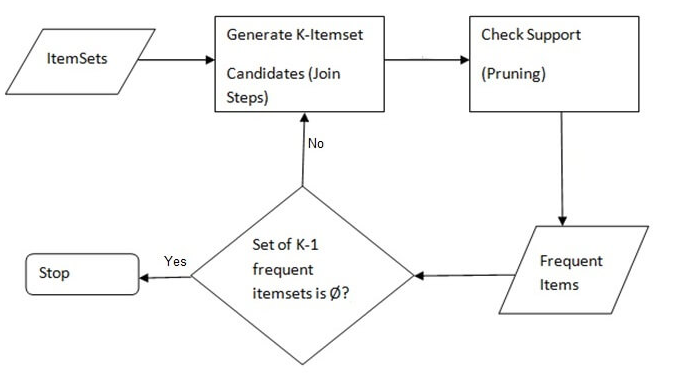
\includegraphics[scale=0.5]{/home/boukala/Bureau/Memoire/figures/diagramme2.png}
\caption{Processus de l'algorithme Apriori}
\end{center}
\end{figure}

L'exemple suivant illustre le fonctionnement de l'algorithme ci-dessus : 

\begin{figure}[h!]
\begin{center}
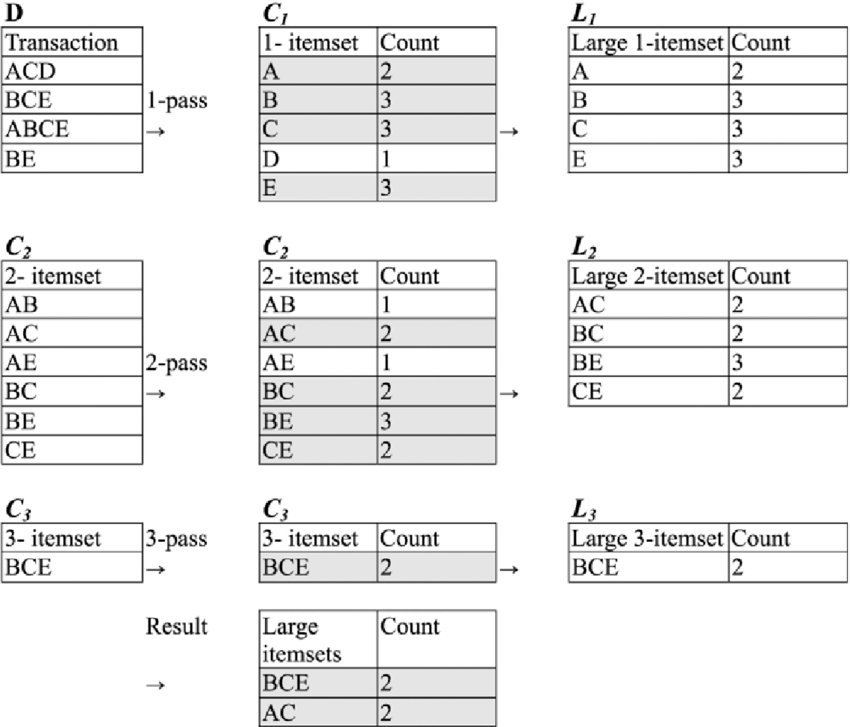
\includegraphics[scale=0.5]{/home/boukala/Bureau/Memoire/figures/deroulementAlgo2.png}
\caption{Exemple de l'algorithme Apriori}
\end{center}
\end{figure}





\paragraph{}
Après avoir déroulé un exemple de l'algorithme, nous proposons le pseudo code suivant :
\paragraph{} 
Le pseudo code suivant permet d'extraire les concepts de l'ontologie cible : 

\begin{figure}[h!]
\begin{center}
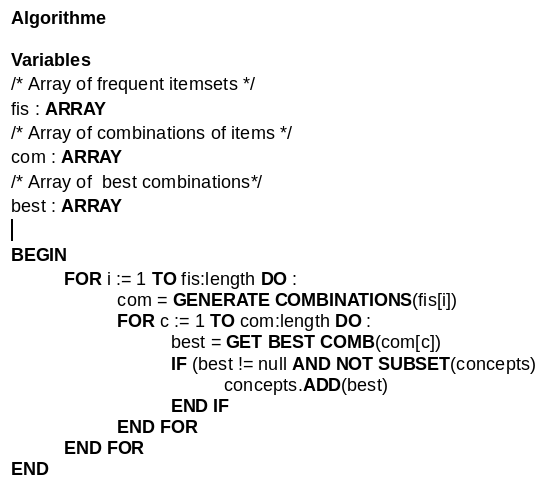
\includegraphics[scale=0.6]{/home/boukala/Bureau/Memoire/figures/algo2.png}
\end{center}
\end{figure}


\paragraph{}
Après avoir trouvé les concepts de l'ontologie, nous formons des paires de concepts et cherchons la présence d'éventuelles relations entre les paires formées.

\subsubsection{Discussion}

\paragraph{}
Apriori est un algorithme très utilisé dans le monde de l'informatique et plus particulièrement dans l'analyse et fouille de données.
Cela est justifié par le fait qu'il s'agisse d'un algorithme assez intuitif, facile à programmer dans n'importe quel langage et offrant la possibilité de faire de la programmation parallèle et des algorithmes répartis.
\paragraph{}
Néanmoins, Apriori présente quelques limitations. Ces dernières sont généralement liées à la densité des documents.\\
Nous citons à titre d'exemple un document possédant  104 1-item fréquents.\\
Ces derniers vont générer 107combinaisons possibles de 2-items fréquents.\\
Par conséquent, le processeur sera très vite surchargé de traitements.

\subsection{Conclusion}
\paragraph{}
Au cours de ce chapitre, nous avons pu explorer deux architectures (méthodes) permettant la mise en oeuvre d'un moteur de recherche sémantique.
\paragraph{}
Ce moteur de recherche a comme particularité d'être basé sur des ontologies générées automatiquement à partir d'un corpus de documents.
\paragraph{}
Les deux méthodes exposées apportent toutes les chances pour produire une implémentation de moteur de recherche sémantique intéressante.
\paragraph{}
Chacune des deux présente des avantages et des inconvénients selon le contexte d'application, de l'approche adoptée, ainsi que du nombre d'itérations par processus.
\paragraph{}
Dans le chapitre suivant, nous proposons une approche personnelle de résolution de la problématique.


\chapter{Cas d'étude du moteur de recherche sémantique des assurances}

\section{Introduction}

\paragraph{}
Le domaine des assurances se voit attribuer de plus en plus d'importance ces dernières années et ce, en raison des différents dangers auxquels l'humain est exposé quotidiennement.
\paragraph{}
A cet effet, nous avons choisi de nous intéresser aux moteurs de recherches sémantiques, rendant la recherche plus pertinente et précise.
\paragraph{}
Toutefois, un tel moteur de recherche requiert l'utilisation d'une ontologie de domaine. Il s'agit de Insurance ontology dans notre cas. 
\paragraph{}
Au cours de ce chapitre, nous détaillons les éléments de la solution que nous proposons, et dont l'implémentation sera présentée juste après.

\section{Acquisition des données}

\paragraph{}
Dans le but de rendre la recherche sémantique riche et précise, il est nécessaire que l'ontologie générée automatiquement soit bien détaillée.\\
Ainsi, nous avons choisi d'utiliser un corpus avec un nombre important de documents. Ces derniers ont tous été extraits de l'ACR8 (Réseau d'AXA France Transports) pour les raisons suivantes : 
\paragraph{}
Les documents présents dans l'ACR8 sont dépourvus de toute structure.
En effet, s'agit de documents textuels simples, non balisés.\\
Il s'agit généralement de clausiers, conditions générales, conditions particulières, guides de souscriptions. Tous liés au domaine des assurances.
\paragraph{}
Enfin, l'application que nous souhaitons mettre en place est destinée à AXA France. Ainsi, l'apprentissage des ontologies serait plus significatif en utilisant les données AXA.

\section{Etude de l'ontologie pré-existante “Insurance”}
\paragraph{}
Insurance est une ontologie de domaine développée par le groupe de recherche “E-Business Web Science”. \\
Cette ontologie permet de décrire des informations liées aux produits d'assurance que les clients trouvent sur le marché.\\
Nous citons comme informations présentes dans cette ontologies : \\

\begin{itemize}

\item \textbf{Object : }Permettant de décrire le produit d'assurance proposé.\\
\item \textbf{Agent : }Représente la compagnie d'assurance mettant à disposition le produit décrit dans Object.\\
\item \textbf{Offer : }Il s'agit de l'offre du produit proposé aux clients.\\
Concepts et relations


\paragraph{}
La figure \ref{exempleOnto} permet d’illustrer l’ontologie décrite ci-dessous en RDF/XML : 

\begin{figure}[h!]
\begin{center}
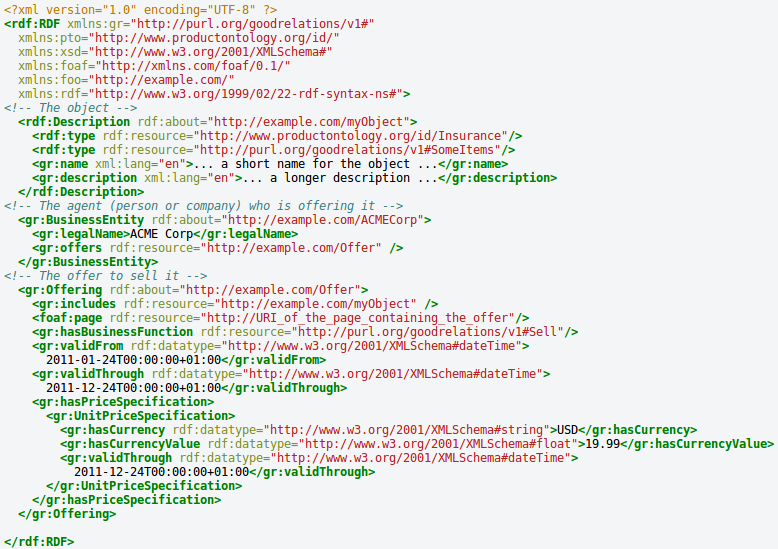
\includegraphics[scale=0.6]{/home/boukala/Bureau/Memoire/figures/rdfinsurance.png}
\captionof{figure}{Ontologie Insurance en RDF/XML}
\label{exempleOnto}
\end{center}
\end{figure}



\end{itemize}

\paragraph{}
Comme indiqué dans le chapitre précédent, toute ontologie est formée d'un ensemble de concepts et de relations permettant de lier deux concepts.
\paragraph{}
L'ontologie \textbf{“Insurance”} est formée des concepts décrits dans le tableau \ref{tableConcept} : 

\begin{figure}[h!]
\begin{center}
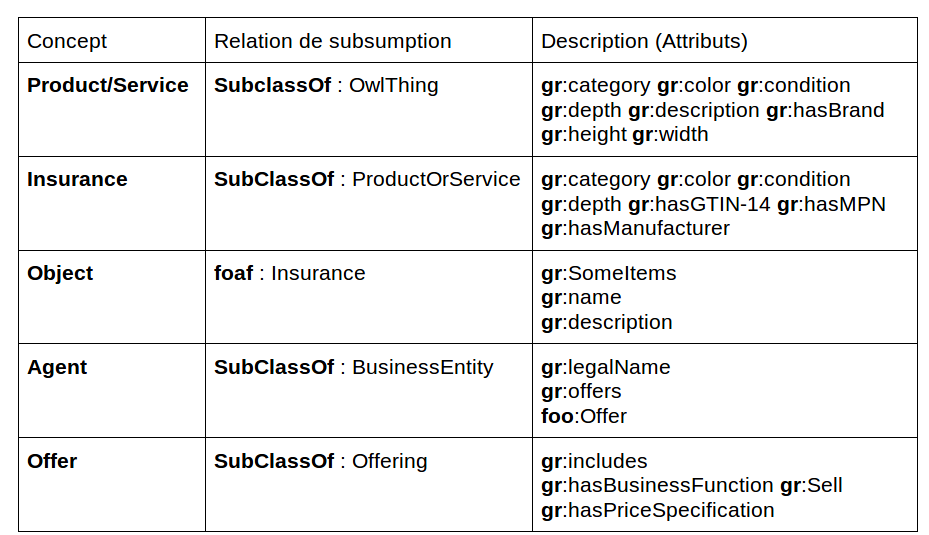
\includegraphics[scale=0.44]{/home/boukala/Bureau/Memoire/figures/tableauConcepts.png}
\captionof{table}{Concepts de l'Ontologie Insurance}
\label{tableConcept}
\end{center}
\end{figure}

\paragraph{}
L'ontologie possède aussi un ensemble de relations que nous détaillons dans le tableau \ref{tableRelation} : 

\begin{figure}[h!]
\begin{center}
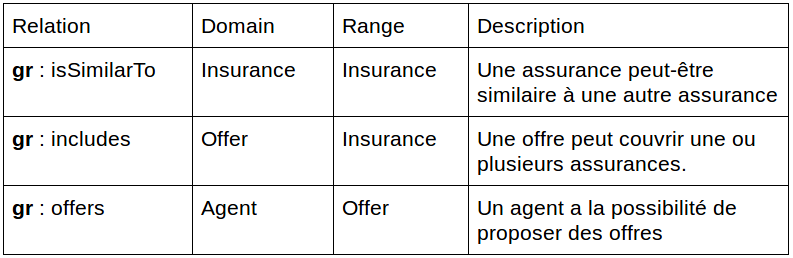
\includegraphics[scale=0.44]{/home/boukala/Bureau/Memoire/figures/TableRelations.png}
\captionof{table}{Relations de l'Ontologie Insurance}
\label{tableRelation}
\end{center}
\end{figure}


\paragraph{}
Après avoir explicité les différents éléments constituant l'ontologie Insurance. 
Nous remarquons que cette dernière répond essentiellement à la description des produits d'assurances. 
\paragraph{}
Il est important de noter qu'un grand nombre de Concepts et Relations est manquant dans cette ontologie par exemple : Les informations sur les clauses et tarifs nationaux.
\paragraph{}
C'est pour cette raison qu'il a été décidé de migrer vers une nouvelle ontologie.\\
Cette nouvelle ontologie est générée automatiquement à partir de la bibliothèque de documents de la branche Transports d'Axa France, et ce dans le but de garantir une meilleure cohérence entre le contenu des documents et l'ontologie générée.

\section{Solution appliquée pour la création automatique des ontologies}
\paragraph{}
Après avoir argumenté sur la nécessité de créer une ontologie propre au contexte auquel nous nous référons, nous présentons la solution d'automatisation basée sur l'architecture suivante : 

\begin{figure}[h!]
\begin{center}
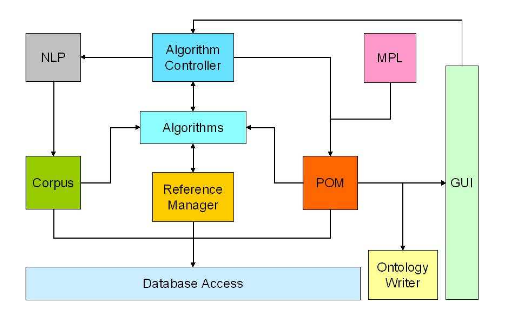
\includegraphics[scale=0.6]{/home/boukala/Bureau/Memoire/figures/architecture2.png}
\captionof{figure}{Génération automatique des Ontologies}
\end{center}
\end{figure}



 
\paragraph{}
Dans ce qui suit, nous détaillons chaque module de cette architecture.

\subsection{Le modèle d'ontologie probabiliste}

\paragraph{}
Il s'agit d'une collection de primitives de modélisation instanciées indépendantes d'un langage de représentation d'ontologies.\\
Les primitives sont généralement les suivantes : \\ 
\begin{itemize}

\item Concepts (Class)\\
\item Concept inheritance (SubClassOf)\\
\item Concept instanciation (InstanceOf)\\
\item Properties/Relations (Relation)\\
\item Domain / Range\\

\end{itemize}

Notons que cette liste n'est pas exhaustive et que nous pouvons intégrer de nouvelles primitives si cela est nécessaire.\\
A partir d'un document non structuré, l'ensemble des primitives est généré automatiquement.\\
Chaque primitive est ensuite représentée en langage ontologique.\\

L'avantage d'utiliser un tel modèle réside dans le fait que chaque primitive générée automatiquement est accompagnée d'un indicateur de pertinence. \\
Cet indicateur représente la probabilité que la primitive associée soit une instance de l'ontologie qui sera créée par la suite.\\
On pourra de ce fait définir un seuil permettant de décider si la primitive est acceptée dans l'ontologie cible.
\paragraph{}
Un autre avantage en utilisant une telle solution concerne la mise à jour de l'ontologie lors de la modification ou l'ajout d'un document.\\En effet, un changement au niveau du corpus implique l'ajout de nouvelles primitives au niveau du POM et la mise à jour de l'indicateur de présence.

\subsection{Découverte du changement des données}
\paragraph{}
Comme indiqué dans le paragraphe précédent, les documents présents dans le corpus peuvent être modifiés.
Suite à ces modifications, il est nécessaire que l'ontologie générée automatiquement soit en cohérence avec les documents présents.
\paragraph{}
C'est au module \textbf{“Data-driven change discovery”} d'intervenir afin de palier à une telle problématique.\\
Data-driven change discovery fournit les méthodes qui assurent l'adaptation de l'ontologie aux changements.\\
Les avantages de ce modules sont les suivants : \\

\begin{enumerate}
\item Utilisation d'un système de traçage, permettant de mettre en relief les modifications subies par l'ontologie.\\
\item Optimisation des temps de traitements car les documents formant le corpus ne sont pas tous parcourus.\\ \item Seuls les documents modifiés seront pris en considération.\\
\end{enumerate}
\paragraph{}
L'utilisation d'un tel modèle requiert le traçage de toutes les modifications effectuées sur les documents, ainsi que sur les ontologies.
\paragraph{}
De manière formelle, il s'agit de représenter la mise à jour de la manière la plus explicite, à savoir, en mettant en relief l'état initial (avant la modification), la modification effectuée (Ajout, suppression ou correction), ainsi que l'état final, que nous désignons “la cible”.
\paragraph{}
Le même processus sera appliqué lors de la modification automatique ou semi-automatique de l'ontologie.
\paragraph{}
Naturellement, ces changement seront accompagnées par la modification du POM, afin de garantir des résultats cohérents et conformes.

\paragraph{}
Notons à titre d'exemple, la modification du fichier 7471664.txt comme indiqué sur la capture d'écran ci-dessus.\\


\begin{figure}[h!]
\begin{center}
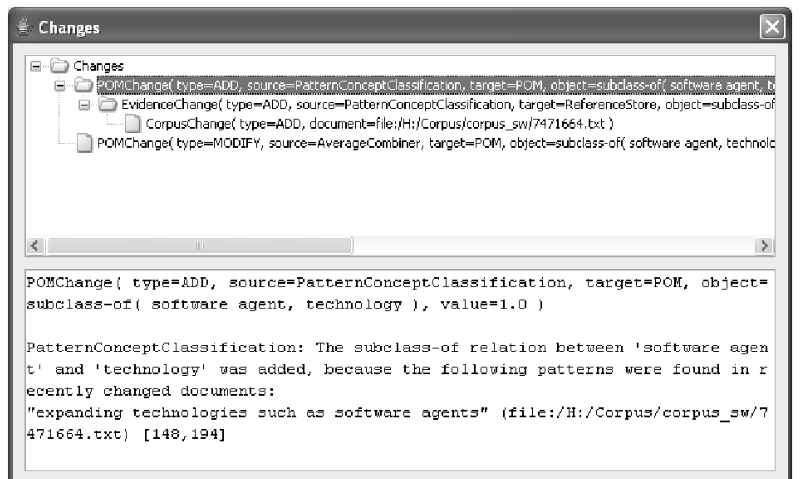
\includegraphics[scale=0.5]{/home/boukala/Bureau/Memoire/figures/pom.png}
\captionof{figure}{Marquage des entités grammaticales}
\end{center}
\end{figure}



Cette modification a conduit à l'ajout d'une nouvelle relation entre les deux concepts “software agent” et “technology”.\\


Cette modification sera par la suite présente dans l'ontologie mise à jour.\\
Enfin, notons que le POM a également subi des changements.


\subsection{Traitement du langage naturel (NLP)}
\paragraph{}
Il existe plusieurs applications dans le Web sémantique permettant l'apprentissage automatique des ontologies à partir d'un texte brut.
\paragraph{}
Ces applications se basent essentiellement soit, sur des analyses linguistiques ou bien sur la Machine Learning.
Dans notre étude, nous avons choisi de combiner ces deux pratiques, et ce dans l'optique de saisir les avantages de chacune et offrir de meilleurs résultats.\citep{nlp}
\paragraph{}
Dans ce qui suit, nous abordons la problématique liée à l'extraction automatique des concepts désignés par plusieurs mots (renvoyant à une même entité).


\subsubsection{L'approche C-value}
\paragraph{}
C-value est une méthode indépendante du domaine textuel étudié. Elle prend en entrée un ensemble de documents et renvoie en sortie une liste de concepts candidats.
\paragraph{}
La liste résultante énumère les concepts extraits, du plus fréquent (pertinent) au moins fréquent. Vient ensuite le rôle de l'expert du domaine, qui procède à l'étude des concepts extraits de haut en bas, dans le but de valider la pertinence de ces derniers quant à l'ontologie cible.
\paragraph{}
La méthode C-value combine un aspect linguistique et statistique à la fois.
\paragraph{}
La partie linguistique permet de baliser le texte en termes et d'effectuer un ensemble de filtrages. 
\paragraph{}
Quant à la partie statistique, elle assigne à chaque sous-chaîne du document une mesure statistique liée à la pertinence de la sous-chaîne de caractères.\\
Cette mesure est appelée “C-value”

\subsubsection{1. La partie linguistique}
\paragraph{}
Le module linguistique comprend les éléments suivants : \\
\begin{itemize}
\item Le marquage des informations du corpus\\
\item Le filtrage des informations marquées\\
\item La stop-list\\

\end{itemize}


\subsubsection{Le marquage des informations du corpus}
\paragraph{}
Chaque mot du corpus donné en entrée est assigné à une entité grammaticale.\\
Une entité grammaticale peut-être un nom, un adjectif, un verbe, une préposition un complément d'objet … .
\paragraph{}
Cette étape est un nécessaire pour accomplir la prochaine étape car le filtrage requiert l'information grammaticale des mots du corpus.
\paragraph{}
Plusieurs algorithmes sont proposés dans la littérature. Dans notre étude, nous avons choisi d'utiliser le langage de programmation Python, mettant à disposition la bibliothèque nltk.\\
Pour chaque mot du corpus donné en entrée, une entité grammaticale est automatiquement renseignée. \\ \\
Le code suivant permet d'effectuer un tel traitement : 
\begin{verbatim}
import nltk
tokens = nltk.word_tokenize("Can you please buy me an Arizona Ice tea ?")
\end{verbatim}

Le résultat obtenu est le suivant : 

\begin{figure}[h!]
\begin{center}
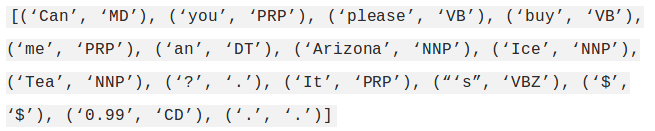
\includegraphics[scale=0.6]{/home/boukala/Bureau/Memoire/figures/grammaire.png}
\captionof{figure}{Marquage des entités grammaticales}
\end{center}
\end{figure}

Le tableau suivant définit chacun des acronymes utilisés : 
\\

\begin{table}[h!]
\centering
\begin{tabular}{| l | l |}
 \hline
 Acronyme & Définition \\
 \hline
 CC & Conjonction de coordination \\
 \hline
 PRP & Pronom personnel \\
 \hline
 VB & Verbe \\
 \hline
 NN & Nom \\
 \hline
\end{tabular}
\caption{Définition des acronymes utilisés}
\end{table}









\subsubsection{Le filtre linguistique}

\paragraph{}
Il s'agit de l'élément permettant de valider la présence d'un mot dans l'ontologie cible selon sa pertinence.\\ 
L'utilisation d'un filtre linguistique est nécessaire pour éviter la présence de mots tels que  : “est un”, “de la” … 
\paragraph{}
De manière générale, les éléments de l'ontologie sont souvent représentés par des noms, adjectifs et des prépositions. Les autres mots sont quant à eux exclus.
\paragraph{}
Il existe plusieurs catégories de filtres, allant du plus restreint au plus large.\\
Prenons à titre d'exemple un filtre prenant en considération que les entités grammaticales : Nom.\\
Ce filtre est désigné dans notre étude par l'expression régulière suivante : 
$$(Nom)+ $$

Ce filtre a comme particularité d'être très restreint.\\

La liste des termes extraite possède un taux de précision très élevé. En revanche, le taux de rappel est quant à lui très faible. \\

D'autres filtres sont proposés dans la littérature, permettant d'obtenir des résultats différents, nous citons : \\
\begin{itemize}
\item \textit{(Nom)+(Nom)} \\
\item \textit{(Adj | Nom)+} \\
\item \textit{(Adj | Nom)+| (Adj | Nom)*} \\
\end{itemize}

Le choix d'utilisation d'un filtre se fait en fonction de l'objectif de l'extraction à effectuer.

\subsubsection{La stop-list}

\paragraph{}
La stop-list est une liste de mots ne devant pas apparaître dans l'ensemble des mots à extraire.
\paragraph{}
Il s'agit de mots qui ne pouvant pas représenter des termes dans l'ontologie cible. \\
Un exemple de mots figurant dans la stop-list : bien, nombreux, bon, juste …. 


\subsubsection{2. La partie statistique}
\paragraph{}
Après avoir effectué un filtrage linguistique des documents constituant le corpus,
seuls les mots susceptibles d'être des termes seront pris en considération lors de l'étape statistique.
\paragraph{}
Comme décrit dans l'idée générale de l'approche adoptée, le paramètre C-value est calculé pour chaque mot rencontré.\\
Ce paramètre permet de classer les mots présents en fonction de leur pertinence dans le corpus.\\
C-value est calculé à l'aide des caractéristiques suivants : \\
\begin{itemize}

\item a. La fréquence totale des occurrences de la chaîne candidate dans le corpus\\
\item b. La fréquence de la chaîne candidate par rapport aux autres termes candidats\\
\item c. Le nombre de termes candidats\\
\item d. La longueur de la chaîne candidate (en nombre de mots)\\


\end{itemize}


\subsubsection{a. La fréquence totale des occurrences de la chaîne candidate dans le corpus}

Permet de calculer l'indicateur statistique $termhood$ à l'aide de la formule suivante:
\begin{equation}
termhood(a) = f(a)
\end{equation}

$a$ : représente une chaîne candidate\\
$f(a)$ : représente la fréquence de l'occurrence de a dans le corpus\\

Cette mesure produit de très bons résultats étant donné que les termes ont tendance à apparaître de manière assez fréquente dans les documents.\\
Prenons à titre d'exemple, un ensemble de documents tirés du domaine des assurances, constitué de 800 000 mots.\\ Le mot “police” apparaît 2 084 fois, ce qui est significatif.
\paragraph{}
Bien entendu, il existe des termes significatifs quant à l'ontologie cible, mais qui n'apparaissent pas beaucoup.
\paragraph{}
Il existe aussi un autre problème lié aux mots composés tel que : responsabilité civile environnementale.\\
En effet, lorsqu'on considère les mots responsabilité, civile et environnementale, séparés, ces derniers ne peuvent représenter une vraie entité dans le domaine des assurances.
\paragraph{}
C'est à partir de cette réflexion que l'idée de considérer la chaîne candidate par rapport aux autres chaînes est apparue.

\subsubsection{b. La fréquence de la chaîne candidate par rapport aux autres termes candidats}
\paragraph{}
L'idée de cette solution consiste à extraire uniquement une sous-chaîne d'un terme candidat dans le cas où ce dernier apparaît un certain nombre de fois dans le corpus. \\
Ensuite, nous pouvons calculer la valeur du termhood d'une chaîne de la manière suivante :

%termhood(a) = f(a) - b  \sum() f(b)      (Formule 2)
\begin{equation}
termhood(a) = f(a) - b  \sum_{b \in T_a} f(b)
\end{equation}

$a$ : représente une chaîne candidate\\
$f(a)$ : représente la fréquence de l'occurrence de a dans le corpus\\
$Ta$ : représente un ensemble de termes candidats contenant la chaîne $a$\\
$f(a)$ : représente la fréquence de l'occurrence de a dans le corpus\\
$b$ : est un terme candidat\\
$f(a)$ : représente la fréquence de l'occurrence du terme $b$ contenant $a$\\ 
Le problème est encore une fois pas totalement résolu. 
\paragraph{}
Pour mieux comprendre, considérons les deux ensembles de termes extraits du domaine de l'Informatique suivants : 
\paragraph{}
$E1$ :
\begin{itemize}

\item real time clock
\item real time expert system
\item real time image generation
\item real time systems

\end{itemize}

\paragraph{}
$E2$ : 
\begin{itemize}

\item floating point arithmetic
\item floating point constant
\item floating point operation
\item floating point routine

\end{itemize}

\paragraph{}
Dans ce qui suit, nous désignons par l'expression \textbf{“termes imbriqués”}, les mots qui apparaissent dans des termes plus longs.
\paragraph{}
Les deux ensembles précédents contiennent des termes imbriqués.\\
$E1$ contient le terme imbriqué \emph{“real time”}. $E2$ contient le terme imbriqué \emph{“floating point”}.\\
Excepté le terme \emph{“expert system”}, les autres mots ne peuvent être considérés comme des termes.\\
De ce fait, les sous-chaînes peuvent ou ne peuvent pas être considérées comme des termes.\\
Par conséquent, une mesure comme définie dans la formule (2) exclut les termes comme  \emph{“expert system”} si ces derniers n'apparaissent pas dans une autre forme, autre que des termes imbriqués.
\paragraph{}
Afin de répondre à telle problématique, 



\subsubsection{d. La longueur de la chaîne candidate (en nombre de mots)}

\paragraph{}
C'est le dernier paramètre permettant de calibrer la valeur du $C-value$.\\
Il s'agit de la longueur de la chaîne candidate en terme de mots.
\paragraph{}
Étant donné qu'une chaîne de caractères longue a moins de chances d'apparaître de manière fréquente dans un corpus comparé à une chaîne courte. 
\paragraph{}
Le fait qu'une chaîne candidate longue apparaisse n fois dans un corpus est plus important que si une chaîne candidate courte apparaisse aussi $n$ fois.
\paragraph{}
C'est pour cette raison que l'idée de prendre en considération la longueur d'une chaîne candidate a été intégrée lors du calcul du $C-value$.
\paragraph{}
Dès lors que les termes de longueur maximale ne peuvent pas être imbriqués et que certains termes imbriqués ne peuvent être extraits, nous pouvons énumérer deux cas de figures : 

\begin{enumerate}

\item Si a est une chaîne de caractères de longueur maximale ou bien n'est pas considérée comme une chaîne imbriquée, alors la valeur de son termhood est égale à son nombre total d'occurrences.
\item Si a est une chaîne courte, et sous-chaîne d'une autre chaîne longue, alors nous devons calculer sa fréquence en prenant en considération les occurrences d'une chaîne imbriquée ainsi qu'une chaîne indépendante.

\end{enumerate}

La valeur du $termhood$, désigné par $C-value$ est donnée par la formule suivante :
\begin{equation}
C-value = \left\{
  \begin{array}{rcr}
    log_2\vert a \vert \cdot f(a)  \;\;\;\;\;\;\;\;\;\;\;\;\;\;\;\;\;\;\;\;\;\;\;\;\;  \; a \; is \; not \; nested  \\
    log_2\vert a \vert \cdot f(a) - \frac{1}{P(T_a)} \cdot \sum_{b \in T_a} f(b) \;\;\; otherwise \\
  \end{array}
\right.
\end{equation}



$a$ : représente la chaîne candidate\\
$f(.)$ : représente la fréquence d'occurrence dans le corpus\\
$Ta$ : représente un ensemble de termes candidats contenant la chaîne a\\
$P(Ta)$ : représente le nombre de termes candidats\\




\subsection{Algorithme de construction}
\paragraph{}
Dans cette partie, nous décrivons les étapes de l'approche $C-value$ suivies afin de construire une liste de termes candidats à partir du corpus donné en entrée.

\subsubsection{Etape 1}

Comme mentionné précédemment, chaque mot du corpus est assigné à une entité grammaticale.\\
Cette étape est nécessaire avant de lancer le filtrage linguistique.

\subsubsection{Etape 2}

Lors de cette étape, les chaînes qui vérifient le filtrage linguistique sont extraites.\\
Les termes seront ainsi identifiés. La longueur maximale des chaînes extraites dépend des éléments suivants :\\
\begin{itemize}
\item \textbf{Le domaine traité} : par exemple : Dans le domaine des arts, les termes ont tendance à être plus courts que ceux que nous trouvons dans les sciences et technologies.
\item \textbf{Le type de termes acceptés} : par exemple : les termes constitués uniquement de noms. 

\end{itemize}
\paragraph{}
Le processus permettant de retrouver les chaînes de longueurs maximales est le suivant : \\
\begin{itemize}

\item Nous commençons par initialiser la longueur max à une valeur arbitraire assez grande.
\item Recherche de chaînes de caractères vérifiant la condition liée à la longueur max.
\item Si aucune chaîne n'est trouvée, la longueur max est décrémentée de 1.
\item Les instructions 2 et 3 sont répétées jusqu'à ce que l'algorithme trouve une chaîne vérifiant la condition dans l'instruction 2.

\end{itemize}
\paragraph{}
Après avoir suivi ces instructions, une liste pour chaque longueur de chaîne est générée automatiquement. (Une liste pour les bigrammes : chaînes à deux mots, une liste pour les trigrammes : chaînes à trois mots ….).
\paragraph{}
Les listes sont ensuite filtrées par rapport à la stop-list et concaténées dans une seule et même liste.
\paragraph{}
La chaîne la plus longue apparaît en haut de la liste et la plus courte tout en bas.

\subsubsection{Etape 3}



\chapter{Travail et réalisation}

\section{Introduction}
\paragraph{}
Au cours du chapitre précédent, nous avons exposé les méthodes statistiques et linguistiques suivies lors de l'implémentation de notre solution.
\paragraph{}
Ce chapitre est consacré à la présentation du projet réalisé. Il est réparti en deux grandes parties.
\paragraph{}
La première partie met en relief l'ensemble des outils utilisés lors de l'implémentation, ainsi que les caractéristiques de chacun.
\paragraph{}
La deuxième quant à elle, expose la solution développée et les résultats obtenus en l'appliquant dans le domaine des assurances et plus particulièrement sur les documents d'AXA France.

\section{Outil utilisés}
\paragraph{}
Tout développement informatique, quelque soit sa difficulté, requiert l'utilisation d'environnements de développement, de langages de programmation et d'outils de gestion.
\paragraph{}
Pour le développement de notre application, nous avons choisi d'utiliser des outils open source et dont le code est mis à disposition des utilisateurs.
\paragraph{}
Ce qui donne la possibilité de modifier et améliorer les codes sans se soucier des problèmes liés à la redistribution.

\subsection{Le langage Java}
\paragraph{}
Java est un langage de programmation orienté-objet créé en 1995 par Sun Microsystems.
\paragraph{}
Java a comme particularité d'être un langage permettant de développer des applications portables, indépendantes du système d'exploitation. 
\paragraph{}
Java est considéré comme étant le langage le plus riche en terme de bibliothèques et documentation.\\
Il permet de développer des applications desktop à l'aide de Java SE (Standard Edition) et des applications Web avec Java EE (Enterprise Edition).
\paragraph{}
C'est pour ces raisons que beaucoup de développeurs se tournent vers les API Java.\\
En contrepartie, les applications Java connaissent une certaine lenteur au moment de l'exécution.

\subsection{L'API Jena}
\paragraph{}
Jena 2 est la librairie JAVA sous-jacente directe de l'outil SQUIN 3 développé par l'Apache Foundation Software et est maintenant sous Apache Software Licence. 
\paragraph{}
Jena est un ensemble de librairies et d'outils dédiés à la construction d'applications orientées Web sémantique. Parmi ces outils, nous trouvons notamment une API Java open source permettant de manipuler des documents
RDF/RDFS OWL et SPARQL et de raisonner sur des modèles ontologiques à l'aide de moteurs d'inférences. 
\paragraph{}
Jena est très facile à manipuler. Cependant, elle n'est pas exemptée de problèmes comme le fait qu'elle n'accepte pas les ontologies de n'importe quel langue, par exemple : les accents ne sont pas pris en compte, en plus du fait que certaines fonctions ne renvoient pas les résultats escomptés.

\subsection{L'outil de versionnage : Git}
\paragraph{}
Lors de l'implémentation, nous avons eu recours à un outil de versionnage Github, afin de garder un historique des différentes versions commitées.
\paragraph{}
GitHub est un service web d'hébergement et de gestion de développement logiciel. Il possède l'avantage d'assurer un contrôle d'accès et des fonctionnalités destinées à la collaboration comme le suivi des bugs, les demandes de fonctionnalités. GitHub propose des comptes professionnels payants, ainsi que des comptes gratuits pour les projets de logiciels libres.


\subsection{Le langage Python}
\paragraph{}
Comme indiqué précédemment, Java a comme inconvénient d'être relativement lent au moment de l'exécution.
Ce point est assez contraignant, particulièrement lorsque les traitements se font sur des données volumineuses.
Dans notre contexte, les données sont représentées par un corpus de documents contenant chacun minimum 5000 mots.
\paragraph{}
Par conséquent, nous avons choisi de nous pencher vers un autre langage de programmation : Python.
\paragraph{}
Python est un langage de programmation placé sous licence libre. Il est conçu pour optimiser la productivité des programmeurs en offrant des outils de haut 
niveau et une syntaxe simple à utiliser.
\paragraph{}
Il est particulièrement utilisé comme langage de script pour automatiser des taĉhes simples mais fastidieuses. Il possède de nombreuses bibliothèques optimisées destinées au calcul numérique.

\subsection{L'éditeur d'ontologies Protégé}
\paragraph{}
Protégé est un éditeur d'ontologies Open source crée à l'université de Stanford et qui permet de créer, lire et de modifier des ontologies. Il nous permet d'effectuer toutes les opérations nécessaires sur les ontologies tels que la création de classes, de relations, d'attributs et d'individus, et dispose d'un raisonneur qui nous permet de vérifier la cohérence de l'ontologie et de ses individus. 
\paragraph{}
Il existe plusieurs éditeurs d'ontologies, mais notre choix s'est porté sur l'éditeur Protégé et ce,  pour sa capacité de travailler sur des ontologies de grandes dimensions, ainsi que sa popularité d'utilisation.

\subsection{L'environnement de développement Eclipse}
\paragraph{}
Eclipse est un environnement de développement Open source.\\
C'est un environnement de production logicielle s'appuyant principalement sur le Java.\\
Notre choix s'est porté sur cet IDE pour ses fonctionnalités destinées à faciliter la programmation des interfaces graphiques.

\subsection{Le langage de requêtes SPARQL}
\paragraph{}
Après avoir généré l'ontologie automatiquement à partir d'un corpus de documents, nous pouvons extraire une base RDF à l'ontologie.
\paragraph{}
Dans notre étude, nous utilisons le langage de requête SPARQL lors de la recherche dans le moteur implémenté.
\paragraph{}
SPARQL est capable de rechercher des motifs de graphe (graph patterns) obligatoires et optionnels ainsi que leurs conjonctions et leurs disjonctions.
Les résultats des interrogations peuvent être des ensembles de résultats ou des graphes.

\subsection{La Gate 4.0}

\subsection{WordNet}



\section{Travail réalisé}

\subsection{Nettoyage des documents}
\paragraph{}
Avant d'entamer tout mécanisme d'apprentissage d'ontologies sur les documents, il est nécessaire que ces derniers soient assainis.
\paragraph{}
Pour ce faire, nous avons développé des scripts en Python, permettant d'automatiser de tels traitements. \\
Les exemples illustrés dans ce qui suit, prennent tous en entrée le même fichier extrait du réseau Axa France.

\subsubsection{Retrait de tous les chiffres}

Nous commençons dans un premier temps par retirer tous les chiffres présents dans les documents.\\
En effet, les chiffres n'ont aucune pertinence, ni utilité quant à l'ontologie qui sera générée.\\
Pour ce faire, nous avons utilisé le code suivant :

\begin{verbatim}
import re
outputfile = re.sub(r'\d+', '', inputfile)
\end{verbatim}

Notons que cette solution utilise une expression régulière qui supprime tous les nombres.
L'exemple suivant permet d'illustrer le code fourni avec un exemple :


\begin{figure}[h!]
\begin{center}
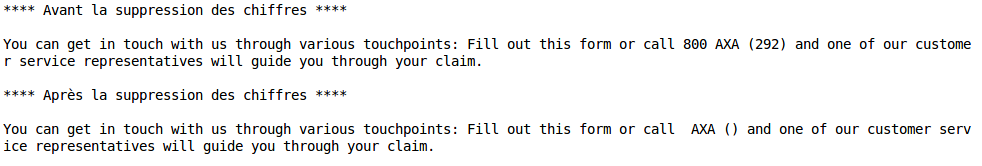
\includegraphics[scale=0.4]{/home/boukala/Bureau/Memoire/figures/chiffres.png}
\captionof{figure}{Suppression des chiffres}
\end{center}
\end{figure}






\subsubsection{Retrait de la ponctuation et des espaces}
\paragraph{}
Dans le but de supprimer la ponctuation, ainsi que les espaces des documents donnés en entrée, nous avons utilisé la portion de code suivante : 
\begin{verbatim}
import string

#Retire la ponctuation
inputfile = inputfile.translate(string.maketrans(“”,””), string.punctuation) 
#Retire les espaces multiple
outputfile = inputfile.strip()
\end{verbatim}

La capture d'écran suivante illustre le traitement effectué :


\begin{figure}[h!]
\begin{center}
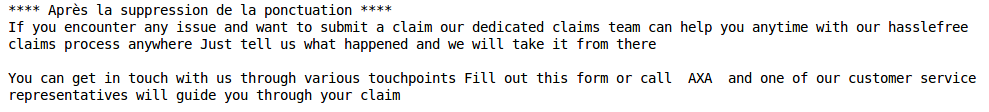
\includegraphics[scale=0.4]{/home/boukala/Bureau/Memoire/figures/ponctuation.png}
\captionof{figure}{Suppression de la ponctuation et des espaces multiples}
\end{center}
\end{figure}



\subsubsection{Suppression des mots communs (Stop words)}
\paragraph{}
Comme indiqué dans l'état de l'art, les textes non structurés sont formés de mots communs appelés Stop words. 
Ces mots n'apportent aucun intérêt lors de l'application des algorithmes de text-mining. 
\paragraph{}
C'est pour cette raison que nous choisissons de les éliminer afin de réduire la taille des documents et se focaliser uniquement sur les mots ayant un intérêt sémantique.
\paragraph{}
Le code suivant permet d'effectuer le traitement décrit précédemment :

\begin{verbatim}
#Spécifie la langue utilisée 
stopwords = set(stopwords.words('english'))
from nltk.tokenize import wordtokenize
tokens = wordtokenize(inputfile)
outputfile= [i for i in tokens if not i in stopwords]
\end{verbatim}

\paragraph{}
La capture d'écran suivante illustre un exemple d'application de l'algorithme sur un texte extrait du réseau Axa.


\begin{figure}[h!]
\begin{center}
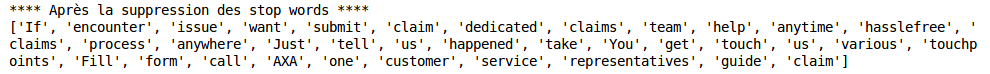
\includegraphics[scale=0.45]{/home/boukala/Bureau/Memoire/figures/removestopwords.png}
\captionof{figure}{Suppression des stop words}
\end{center}
\end{figure}



\paragraph{}
La capture d'écran suivante illustre un exemple des stop words utilisés par l'algorithme :



\begin{figure}[h!]
\begin{center}
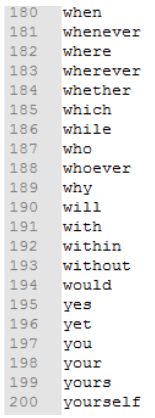
\includegraphics[scale=0.6]{/home/boukala/Bureau/Memoire/figures/stopwords.png}
\captionof{figure}{Illustration de stop words}
\end{center}
\end{figure}






\subsubsection{Stemming}

Cette étape consiste à transformer les mots en stemmer.
Seule la racine du mot est maintenue.\\
Deux algorithmes sont utilisés à cet effet :\\ 
\begin{itemize}
\item Porter stemming algorithm 
\item Lancaster stemming algorithm

\end{itemize}

\paragraph{}
Le code suivant permet d'effectuer un tel traitement : 

\begin{verbatim}
from nltk.stem import PorterStemmer
from nltk.tokenize import wordtokenize

stemmer= PorterStemmer()
inputfile=wordtokenize(inputfile)
for word in inputfile:
   print(stemmer.stem(word))
\end{verbatim}
\paragraph{}
La capture d'écran suivante illustre le traitement décrit avant :


\begin{figure}[h!]
\begin{center}
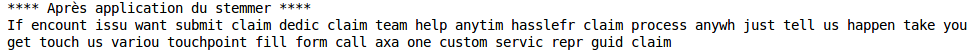
\includegraphics[scale=0.5]{/home/boukala/Bureau/Memoire/figures/stemmer.png}
\captionof{figure}{Application du stemming}
\end{center}
\end{figure}

\paragraph{}
Après avoir appliqué ces traitement préliminaires, le corpus de documents est prêt à être utilisé lors de l'apprentissage automatique de l'ontologie. 

\subsection{Outil de génération automatique des ontologies}
\paragraph{}
Dans le cadre de notre implémentation, nous nous sommes basés essentiellement sur une API développée en Java pré-existante. L'IHM présentée est développée en Swing.
\paragraph{}
Swing est une bibliothèque graphique pour le langage de programmation Java, faisant partie du package Java Foundation Classes (JFC), inclus dans J2SE. Swing constitue l'une des principales évolutions apportées par Java 2 par rapport aux versions antérieures.
\paragraph{}
L'interface graphique se présente comme illustré dans la capture d'écran suivante :

\begin{figure}[h!]
\begin{center}
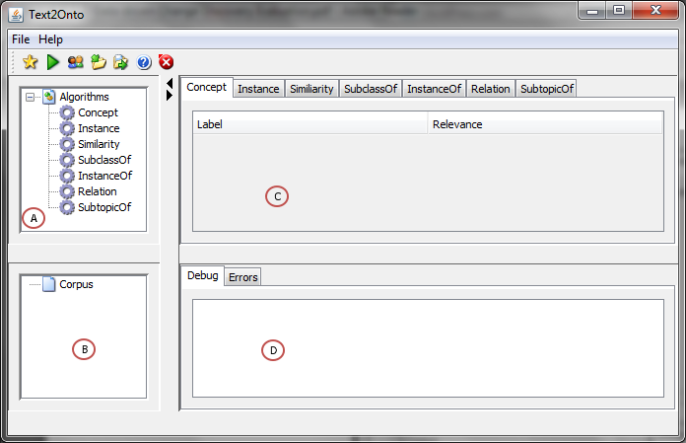
\includegraphics[scale=0.6]{/home/boukala/Bureau/Memoire/figures/text2onto.png}
\captionof{figure}{Interface graphique Text2Onto}
\end{center}
\end{figure}
 

\paragraph{}
Cette interface utilisateur est principalement composée de 4 panels que nous décrivons dans ce qui suit.

\begin{enumerate}
\item \textbf{Le panel A} (marqué par un cercle avec une bordure rouge dans la capture ci-dessus) est une vue Contrôleur dans laquelle nous pouvons spécifier les algorithmes à utiliser et comment combiner les résultats de ces algorithmes.

\item \textbf{Le panel B} permet de gérer le corpus en créant de nouveaux dossiers, ajouter ou supprimer des documents quelque soit leur format (pdf, txt, word … )

\item \textbf{Le panel C} donne un aperçu sur le résultat obtenu après avoir lancé l'étape d'apprentissage d'ontologie à partir des documents formant le corpus.

\item \textbf{Le panel D} est consacré aux messages d'erreur et de débuggage 

\end{enumerate}
\paragraph{}
Après avoir généré les résultats automatiquement, l'expert du domaine a alors la possibilité d'éditer l'ontologie proposée par l'outil en supprimant le bruit (Les concepts et relations non pertinents).\\ L'utilisateur a également la possibilité d'enrichir l'ontologie générée en ajoutant de nouveaux documents dans le corpus.
\paragraph{}
Notons que plusieurs algorithmes d'apprentissage sont proposés à l'utilisateur pour générer l'ontologie.\\
Parmi ces algorithmes, nous citons les 4 algorithmes suivants pour l'extraction des concepts :\\
\begin{itemize}
\item Entropy concept extraction
\item Example concept extraction
\item RTF concept extraction
\item TFIDF concept extraction

\end{itemize}

\paragraph{}
L'utilisateur a la possibilité d'utiliser un seul algorithme à la fois, ou de combiner plusieurs selon sa problématique.
\paragraph{}
A la fin du processus de génération automatique, l'outil propose d'extraire le résultat obtenu sous plusieurs formats : KAON, RDFS or OWL format.
\paragraph{}
Dans notre cas, nous choisissons d'extraire l'ontologie en OWL afin que nous puissions l'importer par la suite dans le framework Protégé.


\subsection{Utilisation du framework \emph{Protégé}}
\paragraph{}
L'ontologie telle que générée automatique requiert des modifications manuelles de la part d'un expert du domaine. Cette contribution se fait dans le but d'aboutir à un modèle ontologique conforme au corpus de documents. 
\paragraph{}
De ce fait, nous commençons par expliquer la démarche suivie lors de l'utilisation de l'éditeur d'ontologies Protégé 2000 pour l'ajout de classes, propriétés et restrictions. \\
Cela est réalisé sur l'ontologie \emph{Insurance} générée automatiquement que nous avons pris comme cas
d'études.
\paragraph{}
Nous commençons par modifier l'ontologie \emph{Insurance} générée précédemment à l'aide de l'éditeur Protégé 2000.\\ Cette modification consiste à rajouter les classes et relations manquantes comme le montre la figure suivante :


\begin{figure}[h!]
\begin{center}
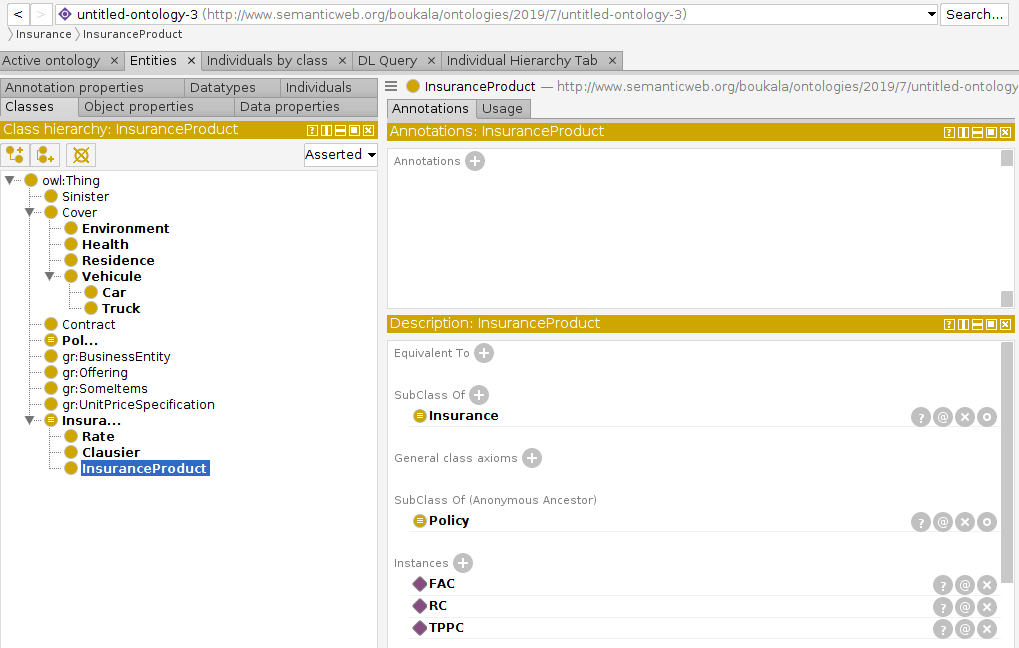
\includegraphics[scale=0.4]{/home/boukala/Bureau/Memoire/figures/protege.png}
\captionof{figure}{Modification de l'ontologie à l'aide de Protégé}
\end{center}
\end{figure}

Parmi les modifications apportées à l'ontologie \emph{Insurance}, je cite : 

\subsubsection{Ajout d'une relation d'équivalence}

Lors de la génération automatique de l'ontologie \emph{Insurance}, deux termes ont été extraits : \emph{Policy} et \emph{Contract}.
Ces deux termes renvoient sémantiquement à un même Concept.\\
Ainsi, j'ai pris le soin d'ajouter une relation  d'équivalence entre ces deux termes, à l'aide de \emph{Protégé}.\\
La capture d'écran suivante permet d'illustrer le résultat obtenu au niveau de l'ontologie Insurance après modification : 

\begin{figure}[h!]
\begin{center}
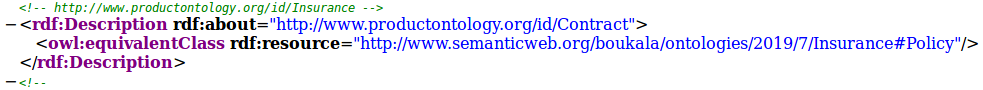
\includegraphics[scale=0.45]{/home/boukala/Bureau/Memoire/figures/equivalence.png}
\captionof{figure}{Insertion d'une relation d'équivalence entre \emph{Contract} et \emph{Policy}}
\end{center}
\end{figure}


\subsubsection{Ajout d'une propriété \emph{InverseOf}}
Après avoir examiné l'ontologie générée automatiquement, j'ai noté la présence de deux relations : \emph{gr:Offers} et \emph{gr:Offered}.\\
La relation \emph{gr:Offers} est formée de la manière suivante : 

\begin{figure}[h!]
\begin{center}
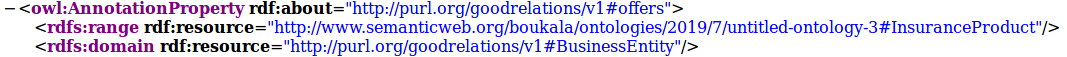
\includegraphics[scale=0.45]{/home/boukala/Bureau/Memoire/figures/offers.png}
\captionof{figure}{Relation \emph{gr:Offers} en OWL.}
\end{center}
\end{figure}

La relation \emph{gr:Offered} est quant à elle formée comme suit : 

\begin{figure}[h!]
\begin{center}
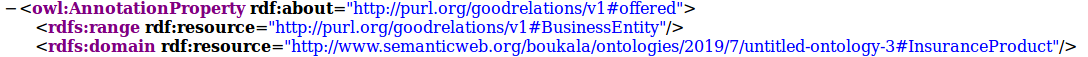
\includegraphics[scale=0.45]{/home/boukala/Bureau/Memoire/figures/offered.png}
\captionof{figure}{Relation \emph{gr:Offered} en OWL.}
\end{center}
\end{figure}

Notons que ces deux relations possèdent des domaines et ranges inversés.\\

De ce fait, j'ai ajouté une propriété \emph{inverseOf} aux deux relations afin de les lier sémantiquement.\\
L'ajout d'une telle propriété a été effectué à l'aide de Protégé et a permis d'obtenir le résultat suivant : 

\begin{figure}[h!]
\begin{center}
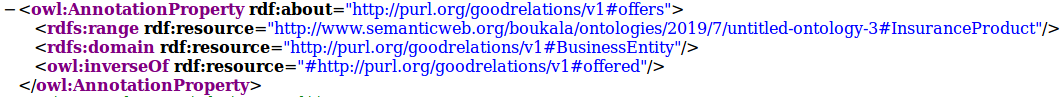
\includegraphics[scale=0.45]{/home/boukala/Bureau/Memoire/figures/inverse.png}
\captionof{figure}{Ajout de la propriété \emph{InverseOf}.}
\end{center}
\end{figure}
\paragraph{}
Après avoir édité l'ontologie \emph{Insurance} à l'aide de Protégé, cette dernière est prête à être utilisée par le moteur de recherche que j'ai développé pour répondre à la problématique de mon mémoire.


\subsection{Insurance : Moteur de recherche sémantique pour les assurances}

\paragraph{}

Le but ultime des travaux exposés précédemment est de pouvoir créer un moteur de recherche sémantique spécialisé dans le domaine des assurances. 

\paragraph{}

Pour ce faire, j'ai développé une application Java dont l'interface graphique est implémentée à l'aide de JavaFX.\\

La figure \ref{recherche} illustre le travail réalisé : 

\begin{figure}[h!]
\begin{center}
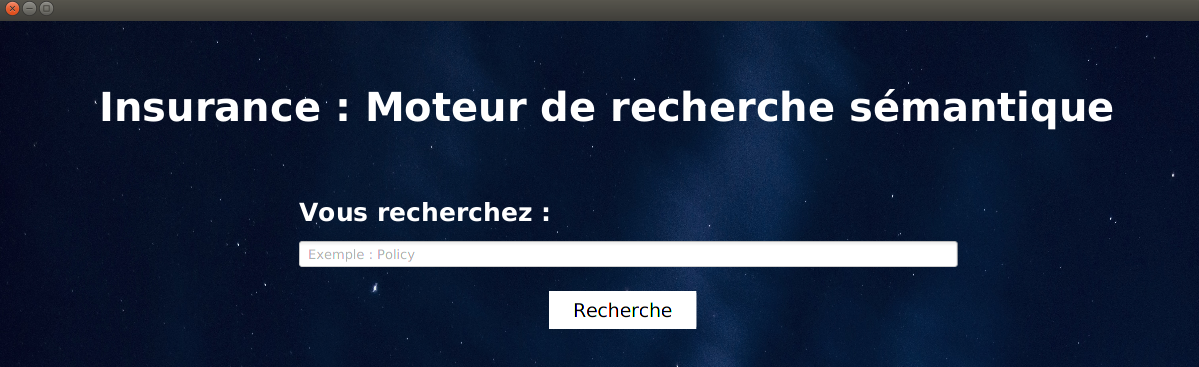
\includegraphics[scale=0.4]{/home/boukala/Bureau/Memoire/figures/recherche.png}
\captionof{figure}{Moteur de recherche \emph{Insurance}}
\label{recherche}
\end{center}
\end{figure}

L'application offre une interface graphique intuitive, ergonomique et facile à manipuler.

\paragraph{}
Dans le cadre d'une recherche sémantique, l'utilisateur renseigne un mot clé dans le champ qui lui est attribué.\\
Ce dernier devra ensuite cliquer sur le bouton \textbf{Recherche} afin de lancer la recherche.

\paragraph{}
Les résultats de la recherche sont ensuite affichés comme suit : 

\begin{figure}[h!]
\begin{center}
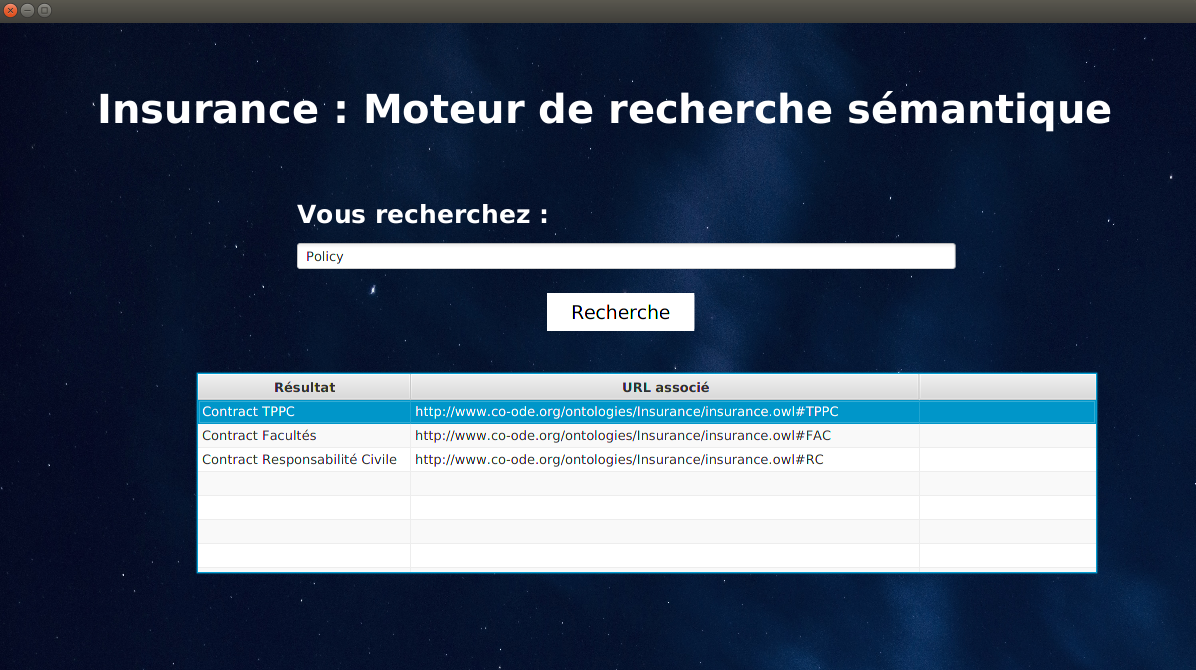
\includegraphics[scale=0.4]{/home/boukala/Bureau/Memoire/figures/resultat.png}
\captionof{figure}{Résultats de la recherche sémantique}
\label{resultat}
\end{center}
\end{figure}

Il est à noter que la capture d'écran précédente illustre un cas concret de recherche sémantique.

\paragraph{}
En effet, lorsque l'utilisateur a introduit le mot clé \textbf{Policy}, il a obtenu des résultats contenant le terme \textbf{Contract} car les deux concepts \textbf{Policy} et \textbf{Contract} sont considérés comme équivalents dans l'ontologie \emph{Insurance}.

\paragraph{}
Par conséquence, le moteur de recherche a utilisé l'expression logique $$Policy \equiv Contract$$
Et a permis de déduire que tous les résultats répondant au mot clé \textbf{Contract}, répondent aussi au mot clé \textbf{Policy} et réciproquement.

\paragraph{}
Les résultats obtenus sont accompagnés des URI renvoyant vers les documents et pages associés.

\subsubsection{Recherche sémantique des informations}
 
 Lors de la recherche sémantique, j'ai utilisé des requêtes SPARQL permettant d'interroger la base RDF \emph{Insurance}.\\
La requête suivante illustre un exemple de requête utilisée :
\begin{verbatim}
PREFIX foaf: <http://xmlns.com/foaf/0.1/>
SELECT distinct ?key ?label
WHERE
{
?key foaf:name ?label
FILTER regex(?name, str("?"), "i")
}
ORDER BY strlen(str(?name))
\end{verbatim}

Les requêtes SPARQL sont exécutées à l'aide de l'API Jena en Java.

\paragraph{Remarque}

Le \emph{"?key"} représente la chaîne de caractères donnée en entrée pour faire la recherche.

\section{Conclusion}

Au cours de ce dernier chapitre, j'ai exposé le travail réalisé afin de répondre au mieux à la problématique énoncée.
\paragraph{}
J'ai présenté les outils utilisés, en argumentant le choix de ces derniers.\\
J'ai aussi exposé des captures d'écran de l'application développée, en expliquant le fonctionnement de celle-ci. 

\paragraph{}
Le moteur de recherche sémantique développé s'applique essentiellement au domaine des assurances.
Nous pouvons facilement imaginer que ce dernier soit appliqué à d'autres domaines, en appliquant la même procédure sur un corpus de documents de domaine différent.
 












\bibliography{Memoire}

\end{document}